\documentclass{article}

\usepackage{graphicx}
\usepackage{multicol}
\usepackage[latin1]{inputenc} % package caracteres francais
\usepackage[T1]{fontenc}      % package caracteres francai
\usepackage[francais]{babel}  % package caracteres francai
\usepackage{vmargin}
\setmarginsrb{20mm}{20mm}{20mm}{20mm}{0mm}{0mm}{4mm}{8mm}

\begin{document}


%======Page de garde=======
\begin{center}

\includegraphics[width=10cm]{logoULFST.jpg} %l'image est retaill\'ee pour avoir une largeur de 10cm
\end{center}

\begin{center}
\thispagestyle{empty}
{\bfseries \large Master Informatique}
\end{center}

\vspace*{70mm}
\begin{center}
	{\bfseries \Huge Rapport du projet d'initiation \`{a} la recherche}
\end{center}
\vspace*{10mm}
\begin{center}
{\large sujet : Constitution d'une base de cas de corrections du fran\c{c}ais}
\end{center}
\begin{center}
{\large Ann\'ee 2018-2019}
\end{center}



\vspace*{60mm}
\begin{multicols}{2}
\begin{multicols}{2}
	\begin{flushright}
		\`{E}tudiants :
	\end{flushright}
		\vfill\null\columnbreak
	\begin{flushleft}
		Alex Ginestra\newline Christopher Klein
	\end{flushleft}
\end{multicols}
\vfill\null\columnbreak
\begin{multicols}{2}
	\begin{flushright}
		\`{E}quipe :
	\end{flushright}
	\begin{flushright}
		Encadrants :
	\end{flushright}
	\vfill\null\columnbreak
	\begin{flushleft}
	Orpailleur et S\'emagramme\newline Bruno Guillaume, Yves Lepage, Jean Lieber et Emmanuel Nauer
	\end{flushleft}
\end{multicols}
\end{multicols}
\cleardoublepage
\cleardoublepage


%=====Page declaration contre le plagiat=====
\thispagestyle{empty}
\begin{center}
{\bfseries \huge D\'echarge de responsabilit\'e}
\end{center}
\vspace*{10mm}

Nous soussignons Alex Ginestra et Christopher Klein, d\'eclarons avoir pris connaissance de la charte des examens et notamment du paragraphe sp\'ecifique au plagiat.\newline
Je suis pleinement conscient(e) que la copie int\'egrale sans citation ni r\'ef\'erence de documents ou d'une partie de document publi\'es sous quelques formes que ce soit (ouvrages, publications, rapports d'\'etudiant, internet etc...) est un plagiat et constitue une violation des droits d'auteur ainsi qu'une fraude caract\'eris\'ee.\newline
En cons\'equence, je m'engage \`{a} citer toutes les sources que j'ai utilis\'ees pour produire et \'ecrire ce document.
\cleardoublepage


%=====Page remerciements=====
\thispagestyle{empty}
\begin{center}
{\bfseries \huge Remerciements}
\end{center}
\vspace*{10mm}

Tout d'abord, nous tenons \`{a} remercier toute l'\'equipe p\'edagogique du d\'epartement informatique de la facult\'e des sciences et technologies pour les quatre ann\'ees de formation en Master informatique.\newline
J'adresse \'egalement mes remerciements \`{a} toute l'\'equipe Orpailleur et S\'emagramme ainsi qu'aux encadrants Bruno Guillaume, Yves Lepage, Jean Lieber et Emmanuel Nauer pour leur accueil et leur sympathie.

\cleardoublepage


%======Sommaire====== 
\begin{center}
{\bfseries \huge Sommaire}
\end{center}
\tableofcontents


\setcounter{page}{3}

\cleardoublepage

%=====Rappel du sujet====
\begin{center}
{\bfseries \huge Rappel du sujet}
\end{center}

\vspace*{10mm}


{\bfseries Probl\'ematique de recherche : }
\newline
\vspace*{2mm}

Le raisonnement \`{a} partir de cas (R\`{a}PC) est un raisonnement hypoth\'etique (en g\'en\'eral) qui consiste \`{a} r\'esoudre un nouveau probl\`{e}me (le probl\`{e}me cible, not\'e cible) en s'appuyant sur une base de cas, un cas \'etant la repr\'esentation d'un \'episode de r\'esolution de probl\`{e}me. On appelle cas source un \'el\'ement de la base de cas. Souvent, on repr\'esente un cas source simplement par un couple (srce, sol(srce)) : srce est un probl\`{e}me source, sol(srce) est une solution de ce probl\`{e}me source. Un mod\`{e}le du processus de R\`{a}PC classique comprend deux \'etapes d'inf\'erence : 
Rem\'emoration : un cas source (srce, sol(srce)) jug\'e similaire au probl\`{e}me cible (par exemple, sur la base d'une distance entre probl\`{e}mes) est s\'electionn\'e. 
Adaptation : La solution sol(srce) de ce cas est modifi\'ee en une solution candidate sol(cible) de cible. 

La correction de phrases est la probl\'ematique de la transformation d'une phrase incorrecte (en particulier, grammaticalement) en une phrase corrig\'ee (nous choisirons la langue fran\c{c}aise dans ce travail, m\^eme si la probl\'ematique existe dans toutes les langues). Un cas de correction de phrase est donc un couple (srce, sol(srce)) o\`{u} srce est une phrase incorrecte et sol(srce) une correction de srce. Par exemple, on a les deux cas : 
srce1 = Tu as pas mang\'e. sol(srce1) = Tu n'as pas mang\'e. 
srce2 = Il a recommencer. sol(srce2) = Il a recommenc\'e. 
L'adaptation se fait par des techniques de raisonnement par analogie : la solution sol(cible) est solution d'une \'equation analogique << srce est \`{a} sol(srce) ce que cible est \`{a} y >>. Par exemple, l'adaptation de (srce2, sol(srce2)) \`{a} cible = Tu as manger. consiste \`{a} r\'esoudre Il a recommencer. est \`{a} Il a recommenc\'e. ce que Tu as manger. est \`{a} x qui a pour solution, avec la relation d'analogie utilis\'ee dans le projet, x = Tu as mang\'e., proposition de solution propos\'ee par le syst\`{e}me. 
Sujet : 
Comme pour tout syst\`{e}me \`{a} base de connaissances, la qualit\'e d'un syst\`{e}me de R\`{a}PC d\'epend de celle de son moteur d'inf\'erences mais \'egalement de la qualit\'e de sa base de connaissances, en particulier de sa base de cas. Une bonne base de cas doit avoir plusieurs qualit\'es. Les cas sources doivent \^etre corrects. Elle doit avoir une bonne couverture (et permettre de r\'esoudre correctement une proportion importante de cas). Elle devrait ne pas \^etre trop redondante (certains cas diff\'erents correspondent \`{a} la m\^eme correction). 
Pour cela, on pourra consulter les mouchards d'\'edition de Wikip\'edia pour en extraire des listes de fautes grammaticales ou orthographiques typiques, ainsi que des sites de dict\'ees ou d'orthographe. Il faudra mettre en place les outils de collecte automatiques, param\'etrables en fonction des sites. 
Une autre piste est la mise en place d'un jeu interactif avec un but. Le but est de faire corriger des phrases fautives par les joueurs. La phrase corrig\'ee devrait \'emerger de la majorit\'e des propositions de correction. Les phrases fautives pourraient \^etre extraites de listes d'exemples fautifs, ou produites automatiquement \`{a} partir de patrons pr\'ed\'efinis ou par application de l'analogie sur des cas d\'ej\`{a} collect\'es.
Une courte \'etude bibliographique sur la maintenance de base de cas permettra de sugg\'erer des pistes pour l'acquisition d'une bonne base de cas. Il faudra mettre en place une m\'ethode pour cela, qui pourra s'appuyer sur les sites mentionn\'es ci-dessus.

\cleardoublepage


%===== Introduction ====
\begin{center}
{\bfseries \huge Introduction}
\end{center}

\vspace*{35mm}


Le TAL (traitement automatique des langues) ou TALN (traitement automatique du langage naturel) est un domaine dont le but est de cr\'eer des outils de traitement de la langue naturelle pour diverses applications. Le traitement automatique du langage naturel couvre de tr\`{e}s nombreuses disciplines de recherche. Ces applications servent notamment dans le domaine de la syntaxe, de la s\'emantique, du traitement de la parole ou encore dans le domaine de la fouille de donn\'ees.
\newline

Les premiers travaux remontent en 1950, pendant la guerre froide, ou Alan Turing expose un test, commun\'ement appel\'e le <<test de Turing>>, qui vise \`{a} mesurer la capacit\'e d'un programme informatique \`{a} communiquer avec un humain. Ce test permet de mesurer <<l'intelligence>> d'une machine. Depuis, le traitement automatique des langues a bien \'evolu\'e et est devenu un domaine pluridisciplinaire alliant la linguistique, l'informatique, l'intelligence artificielle pour cr\'eer des applications de plus en plus complexes nous permettant de simplifier nos t\^aches quotidiennes. 
\newline

Un correcteur automatique de la langue est un exemple d'outil utilisant des domaines du traitement automatique des langues. Il utilise des discipline de recherche vari\'es tel que l'analyse syntaxique, la correction orthographique et d'autre plus sp\'ecifique tel que la d\'elimitation de phrase ou la morphologie. Un outil tel que celui-ci est un monstre de conception et de d\'eveloppement et les meilleurs correcteurs automatique connues \`{a} ce jour ont \'et\'e d\'evelopp\'es par des entreprises internationales comme Microsoft, Google ou encore Apple. 
\newline

Contrairement aux cas d\'ecrit pr\'ec\'edemment, notre sujet consiste \`{a} cr\'eer un syst\`{e}me permettant la correction automatique de phrases fran\c{c}aise en s'appuyant sur le raisonnement \`{a} partir de cas (R\`{a}PC). Pour r\'epondre \`{a} cette probl\'ematique, nous allons tout d'abord introduire le raisonnement \`{a} partir de cas et expliquer comment il va nous permettre de corriger des phrases. Puis nous aborderons une partie plus pratique o\`{u} nous d\'etaillerons les diff\'erentes \'etapes permettant de r\'esoudre notre probl\'ematique. Nous parlerons ensuite des r\'esultats obtenus suite \`{a} nos d\'eveloppements et finirons par introduire les suites possibles \`{a} notre projet.

\cleardoublepage


%===== 1ere partie ====
\section{Analyse du probl\`{e}me et organisation}

%===== 1ere sous partie ====
\subsection{Raisonnement \`{a} partir de cas}
Le raisonnement \`{a} partir de cas (not\'{e} R\`{a}PC) est un raisonnement semblable a celui des humain qui consiste \`{a} r\'{e}soudre des probl\`{e}mes de la vie quotidienne s'appuyant sur des exp\'{e}riences semblable rencontr\'{e}s par le pass\'{e}. Gr\^ace aux exp\'{e}riences pass\'{e}es d\'{e}j\`{a} r\'{e}solues, nous arrivons \`{a} en d\'{e}duire une solution qui automatiquement s'ajoute \`{a} notre exp\'{e}rience. La reproduction de cet exemple un grand nombre de cas nous permettra d'avoir une exp\'{e}rience telle que nous arriverons \`{a} d\'{e}duire une solution de n'importe quel probl\`{e}me.
\newline
\newline
Nous voyons donc qu'il y a deux principales \'{e}tapes dans ce raisonnement. Premi\`{e}rement, il y a ce qu'on appellera la <<rem\'{e}moration>>, qui est le rapprochement entre notre probl\`{e}me actuel (que nous appellerons probl\`{e}me cible) et un probl\`{e}me qui a d\'{e}j\`{a} \'{e}t\'{e} r\'{e}solu dans le pass\'{e} (qu'on nommera probl\`{e}me source). La seconde \'{e}tape s'appelle l'>>adaptation>>. Ce principe permet d'obtenir une solution de notre probl\`{e}me source en modifiant la solution du probl\`{e}me cible.
\newline
\newline
%==== image ====
\begin{center}
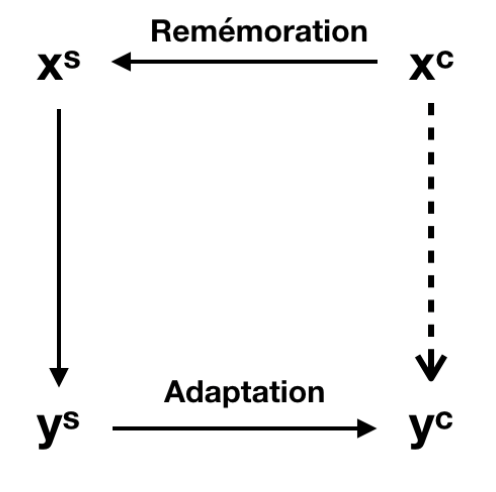
\includegraphics[width=7cm]{img1.png} %l'image est retaill\'ee pour avoir une largeur de 10cm
\end{center}

Nous voyons donc qu'il est possible de r\'{e}soudre des probl\`{e}mes gr\^ace au raisonnement \`{a} partir de cas. N\'{e}anmoins, pour pouvoir les r\'{e}soudre, nous devons avoir des probl\`{e}mes similaire d\'{e}j\`{a} r\'{e}solus. Cet ensemble de couples (probl\`{e}me, solution) r\'{e}solu s'appelle une base de cas. En plus du couple (probl\`{e}me, solution), une explication est ajout\'{e}e et permet d'am\'{e}liorer l'\'{e}tape de la rem\'{e}moration.
\newline
\newline
Voici un exemple de r\'{e}solution de probl\`{e}me gr\^ace au raisonnement \`{a} partir de cas : 
Voici le probl\`{e}me que nous rencontrons (probl\`{e}me cible) : <<Tu n'as pas manger>>.
Nous avons dans notre base de cas un couple tel que celui-ci : <<Il a recommencer>> est le probl\`{e}me source et <<Il a recommenc\'{e}>> est la solution du probl\`{e}me source.
La rem\'{e}moration va donc rapprocher notre probl\`{e}me cible du probl\`{e}me source et en utilisant la solution du probl\`{e}me source ainsi que l'explication, l'Adaptation va pouvoir nous fournir une solution de notre probl\`{e}me cible qui sera <<Tu n'as pas mang\'{e}>>.
\newline
\newline
Pour parvenir \`{a} r\'{e}soudre notre probl\'{e}matique qui est la correction automatique du fran\c{c}ais \`{a} l'aide du raisonnement \`{a} partir du cas, il nous faut donc une base de cas qui permette en th\'{e}orie de corriger toutes les erreurs possible du fran\c{c}ais. En prenant en compte tous les types d'erreurs possibles (grammaire, orthographe, conjugaison, etc.), il y aurait un nombre immense de cas \`{a} d\'{e}finir dans notre base, ce qui est impossible \`{a} construire \`{a} la main. Le but de notre projet est donc de construire une base de cas \`{a} l'aide d'outils diverses et vari\'{e}s qui serait totalement automatis\'{e}e.

\cleardoublepage

%===== 2eme sous partie ====
\subsection{Travail existant}

Une premi\`{e}re piste nous a \'{e}t\'{e} fournie par un groupe d'\'{e}tudiants de L3 de 2017-2018 compos\'{e} de M. Giang, M. Levy, M. Ly, qui avaient travaill\'{e} sur un projet intitul\'{e} Corrector. Le projet consistait \`{a} faire un site Internet capable d'apporter une correction \`{a} une phrase fausse donn\'{e}e en entr\'{e}e. Cette correction devait se faire \`{a} l'aide d'une base de cas qui pouvait s'enrichir avec des interactions humaines (utilisateur/administrateur du site). 
\newline
\newline
Notre d\'{e}but d'\'{e}tude a donc \'{e}t\'{e} guid\'{e} par les moyens mis en {\oe}uvre pour effectuer un remplissage automatique de leur base de cas initiale, et plus particuli\`{e}rement un : les corpus de WiCoPaCo. Le site WiCoPaCo met en libre acc\`{e}s des fichiers au format XML contenant des phrases, ou parties de phrases avec une correction effectu\'{e}e ainsi qu'un commentaire \'{e}ventuel laiss\'{e} par l'auteur de la correction. Ces fichiers sont le r\'{e}sultat des corrections faites par les administrateurs des pages Wikip\'{e}dia, ce qui n\'{e}cessite une correction \'{e}tant donn\'{e} que les contenu des pages est apport\'{e} par des utilisateurs. Les fichiers en question contiennent donc des centaines de milliers de cas compos\'{e}s de la mani\`{e}re suivante : le groupe de phrase avant modification avec la mise en \'{e}vidence de la faute, suivi du m\^eme groupe de phrase avec la correction apport\'{e}e \'{e}galement mise en \'{e}vidence. 
\newline
\newline
L'int\'{e}r\^et principal de ces fichiers \'{e}tant l'\'{e}norme masse de donn\'{e}es qu'ils contiennent, nous permettant ainsi d'en extraire un grand nombre de cas. Cependant, m\^eme si cette solution semble \^etre id\'{e}ale et simple \`{a} mettre en place, il s'av\`{e}re qu'elle est loin d'\^etre parfaite. Car sur ces corrections, une partie \'{e}tant des corrections de contenu, une autre \'{e}tant des reformulations, et bien d'autres types de corrections n'\'{e}tant pas des erreurs de fran
ais mais sont pourtant contenues dans ces fichiers. La probl\'{e}matique de l'\'{e}puration de cette \'{e}norme masse de donn\'{e}es se pose donc.
\newline
\newline
Face \`{a} ce probl\`{e}me, le groupe d'\'{e}tudiants de L3 avait mis en place un script python qui prenait un fichier XML en entr\'{e}e et produisait en fichier CSV en sortie. Le script s'occupait aussi de la suppression de certains cas : les retours en arri\`{e}re. Il ne retenait donc pas les cas qui \'{e}taient des retours sur correction, c'est \`{a} dire lorsque le correcteur transformait une phrase A en phrase B, puis transformait \`{a} nouveau la phrase B en phrase A.
\newline
\newline
C'est donc en reprenant cette base de travail que nous avons d\'{e}but\'{e} notre projet, dans l'optique de pouvoir \'{e}purer cette \'{e}norme masse de donn\'{e}es \`{a} l'aide de filtres pour obtenir uniquement des cas de corrections de langue. 

\vspace*{35mm}


%===== 3eme sous partie ====
\subsection{Mise en place du projet}
Pour mettre en place notre projet, nous avons donc grandement utilis\'{e} le travail d\'{e}j\`{a} effectu\'{e} par nos coll\`{e}gues qui nous ont pr\'{e}c\'{e}d\'{e}s. Nous avons d\'{e}cid\'{e} d'utiliser l'\'{e}norme quantit\'{e} de cas que nous fournissait les fichiers XML de WiCoPaCo pour cr\'{e}er notre base de cas automatique. Ces fichiers regroupant plus de 200 000 cas, elle serait suffisamment cons\'{e}quente pour couvrir un maximum d'erreur de fran\c{c}ais. N\'{e}anmoins, comme cela a ete dit ci dessus, nous ne pouvons pas seulement transform\'{e} ces fichiers directement en une base de cas car un grand nombre de cas ne sont pas utilisable. Nous devons donc reprendre le travail qui a \'{e}t\'{e} fait en amont et continu\'{e} \`{a} filtr\'{e}s les cas jusqu'\`{a} obtenir un ensemble de cas correctes.
\newline
\newline
	\`{a} la suite d'une r\'{e}flexion sur le d\'{e}veloppement de notre projet, nous avons d\'{e}cid\'{e} de ne pas reprendre les travaux effectu\'{e}s par les \'{e}tudiants pr\'{e}c\'{e}dent pour plusieurs raisons : premi\`{e}rement, bien que nous comprenions l'id\'{e}e directrice du d\'{e}veloppement, nous n'avions pas toutes les subtilit\'{e}s pour comprendre parfaitement le code. De plus, nous avions dans l'optique d'impl\'{e}menter plusieurs filtres et que la cr\'{e}ation de ceux-ci soit facile. C'est pourquoi nous nous sommes r\'{e}solues a utilis\'{e} le langage orient\'{e} objet Java pour le d\'{e}veloppement de notre application car c'est un langage que nous avons eu l'habitude de c\^{o}toyer au cours de nos \'{e}tudes, qui permet de lire et d'\'{e}crire des fichiers facilement et qui permet, une fois le projet structur\'{e}, une impl\'{e}mentation simple et rapide de nouvelles fonctionnalit\'{e}s.




\end{document}

